% !TEX root = ./MATH2160.tex
\chapter{Numerical Differentiation and Integration}\label{chapter:Calculus}

Given a differentiable function, we can always find its derivative, although this may not be inviting if the function is complicated. Numerical differentiation approximates the derivative using only function values. Numerical differentiation formul\ae~can be used for solving initial-value problems and other differential equations. Integration is another problem that can be handled numerically only using function values. Numerical integration is clearly useful since there are many functions that cannot be integrated by hand nor analytically by powerful symbolic software, and often the analytical expressions that {\em do} exist are numerically impractical.

\section{Finite Differences}

Given $f\in C^1((a,b))$, recall that:
\[
f'(x) = \lim_{h\to0}\dfrac{f(x+h)-f(x)}{h}.
\]
For a sufficiently small $h$, we can make the approximation:
\[
f'(x) \approx \dfrac{f(x+h)-f(x)}{h}.
\]
Let us study the error in this approximation, which is known as the {\bf first-order forward difference}. From Taylor's remainder theorem, if we assume $f\in C^2((a,b))$:
\[
\left|f'(x) - \dfrac{f(x+h)-f(x)}{h}\right| \le \dfrac{h}{2}\max_{\xi\in(a,b)}|f''(\xi)|.
\]
Since this error term holds for all $x\in(a,b)$, we say that this approximation is of first-order. If we take a small step backward instead, then we arrive at the backward difference formula:
\[
f'(x) \approx \dfrac{f(x)-f(x-h)}{h},
\]
which has the same upper bound on the error as the forward difference.

In many applications, this is not accurate enough. Higher order schemes can be created by ensuring more terms in the Taylor series are removed as $h\to0$ in the formula. Consider the second-order formula created by averaging the forward and backward differences:
\[
f'(x) \approx \dfrac{f(x+h)-f(x-h)}{2h}.
\]
This is called a centered difference scheme. To see this, subtract the Taylor expansions:
\[
f(x\pm h) = f(x) \pm f'(x)h + \dfrac{f''(x)}{2}h^2 \pm \dfrac{f'''(c_\pm)}{6}h^3,
\]
for some constants $c_\pm\in(x,x\pm h)$ to obtain:
\[
\left|f'(x) - \dfrac{f(x+h)-f(x-h)}{2h}\right| = \left|\dfrac{f'''(c_+) + f'''(c_-)}{12}h^2\right| \le \dfrac{h^2}{6}\max_{\xi\in(a,b)}|f'''(\xi)|,
\]
for all $x\in(a,b)$.

It is not difficult to derive a second-order finite difference approximation of the second derivative. Assume that $f\in C^4((a,b))$. Adding the Taylor expansions:
\[
f(x\pm h) = f(x) \pm f'(x)h + \dfrac{f''(x)}{2}h^2 \pm \dfrac{f'''(x)}{6}h^3 + \dfrac{f^{({\rm iv})}(c_\pm)}{24}h^4,
\]
we obtain, after some algebra:
\[
f''(x) \approx \dfrac{f(x+h)-2f(x) + f(x-h)}{h^2},
\]
and indeed the approximation is second-order since:
\[
\left|f''(x) - \dfrac{f(x+h)-2f(x) + f(x-h)}{h^2}\right| = \left|\dfrac{f^{({\rm iv})}(c_+) + f^{({\rm iv})}(c_-)}{24}h^2\right| \le \dfrac{h^2}{12}\max_{\xi\in(a,b)}|f^{({\rm iv})}(\xi)|.
\]

\subsection{Complex Differences}

Consider using the Taylor expansion of $f$ with a small perturbation into the complex plane:
\[
f(x+\i h) = f(x) + \i f'(x)h - \dfrac{f''(x)}{2}h^2 - \i\dfrac{f'''(c)}{6}h^3,
\]
where $c-x\in\i(0,h)$. This expansion motivates the complex finite difference formula:
\[
f'(x) \approx \Im\left\{\dfrac{f(x+\i h)}{h}\right\},
\]
which is second-order since:
\[
\left|f'(x) - \Im\left\{\dfrac{f(x+\i h)}{h}\right\}\right| = \left|\dfrac{f'''(c)}{6}h^2\right| \le \dfrac{h^2}{6}\max_{\xi\in(x,x+\i h)}|f'''(\xi)|.
\]
Using just a single function evaluation in the complex difference formula, we obtain second-order accuracy equivalent to the centered difference formula! Furthermore, as there is no subtraction involved in the complex finite difference formula, we expect the formula to have better numerical stability properties. Indeed, Figure~\ref{figure:FiniteDifferences} shows the resulting error when numerically differentiating $f(x) = e^x$ at $x=1$ using the first- and second-order finite difference formul\ae~and the second-order complex finite difference formula.

\begin{figure}[htbp]
\begin{center}
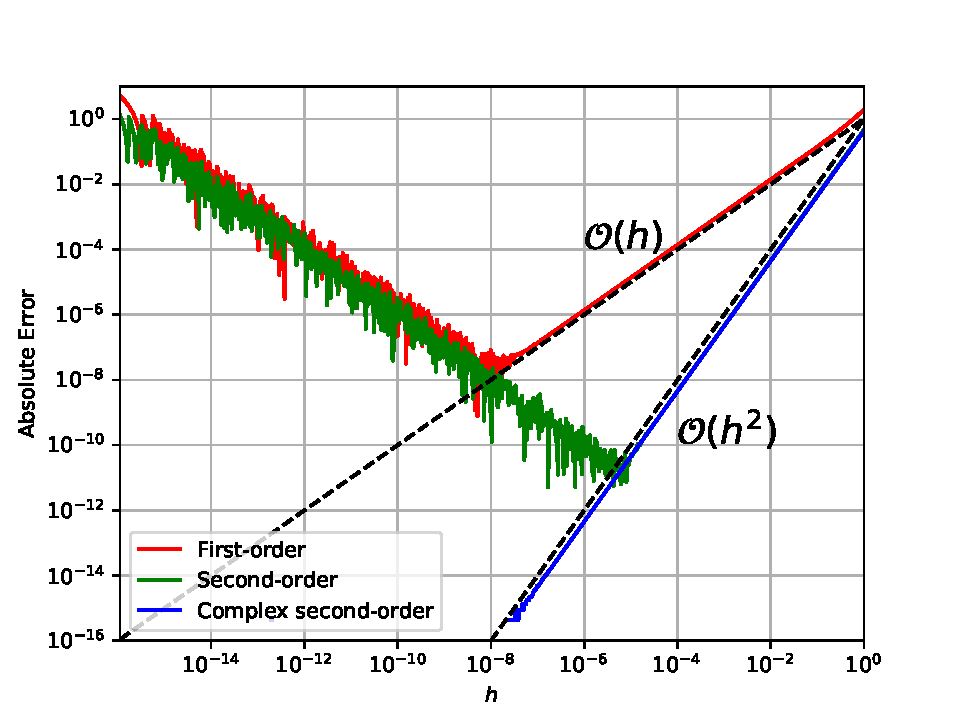
\includegraphics[width=0.65\textwidth]{finitedifferences}
\caption{Comparison of first- and second-order finite difference formul\ae~and the second-order complex finite difference formula for $f(x)=e^x$ at $x=1$. The dashed black lines are representative first- and second-order scalings.}
\label{figure:FiniteDifferences}
\end{center}
\end{figure}

While the complex finite difference formul\ae~are impressive, and relieve the numerical instability of finite difference formul\ae~due to subtractive cancellation, the ability to numerically evaluate a function in the complex plane assumes {\em analyticity}, which is much stronger than the weak assumptions of second- and third-order differentiability. So, any comparison with complex finite differencing is unfair.

\subsection{Dual Numbers and Forward-Mode Automatic Differentiation}

Let $\F$ be the field of real or complex numbers $\R$ or $\C$. Dual numbers extend the field $\F$ with a unit dual $\varepsilon$ to the quotient ring $\D:= \F[\varepsilon]/(\varepsilon^2)$, i.e. the unit dual number satisfies $\varepsilon^2=0$. Thus, it is clear that dual numbers obey the following rules for addition and multiplication:
\[
(a+b\varepsilon) + (c+d\varepsilon) = (a+c) + (b+d)\varepsilon,\quad{\rm and}\quad (a+b\varepsilon)(c+d\varepsilon) = ac + (ad+bc)\varepsilon.
\]
Remarkably, the product of two dual numbers is the product of the two primal components and the dual component can be interpreted as the product rule differentiation formula.
\begin{example}
Let $f(x) = x^2$. Then evaluation at the dual number $x=a+b\varepsilon$ is:
\[
f(a+b\varepsilon) = (a+b\varepsilon)^2 = a^2 + 2ab\varepsilon.
\]
\end{example}
Dual numbers can be interpreted as evaluation at the matrix:
\[
\begin{bmatrix}
a & b\\
0 & a\\
\end{bmatrix},
\]
since this matrix satisfies the addition and multiplication rules of $\D$.
\begin{example}
Let $f(x) = e^x$. The evaluation at the dual number $x=a+b\varepsilon$ can be achieved via the matrix exponential. Since $A:=\diag(a,a)$ and $B:=\begin{bmatrix} 0 & b\\0 & 0\\\end{bmatrix}$ commute, i.e. $AB=BA$, using the property $e^{A+B} = e^Ae^B$, we find:
\[
e^{a+b\varepsilon} = e^{A+B} = e^Ae^B = \begin{bmatrix}e^a & 0\\ 0 & e^a\\\end{bmatrix}\begin{bmatrix}1 & b\\ 0 & 1\\\end{bmatrix} = \begin{bmatrix}e^a & be^a\\ 0 & e^a\\\end{bmatrix} = e^a(1+b\varepsilon).
\]
\end{example}

These simple examples motivate the following definition for evaluation of a function at a dual number.
\begin{definition}
Let $D\subset\F$. Evaluation of $f$ at a dual number $x\in D$ is defined by:
\begin{equation}
f(a+b\varepsilon) := f(a) + \lim_{h\to0}\dfrac{f(a+b\varepsilon h)-f(a)}{h}.
\end{equation}
\end{definition}
When $f$ is differentiable at $a$, we can identify the limit as the derivative:
\[
f(a+b\varepsilon) = f(a) + f'(a)b\varepsilon.
\]

Endowed with only the above properties, dual numbers are a powerful tool for numerical differentiation. In fact, the dual component of the differentiable function $f(a+b\varepsilon)$ {\em is} the function's derivative scaled by $b$, effectively implementing the chain rule differentiation formula since $b$ is allowed to store other differentiation information. Since multiplication of two dual numbers implements the product rule differentiation formula, we have everything we need in order to evaluate complicated derivatives on a computer. In any computer programming language that allows {\em operator overloading}, we can {\em overload} the functions 
\begin{verbatim}
exp(x::Dual) = exp(x.value) * (1 + x.dual * epsilon)
sin(x::Dual) = sin(x.value) + x.dual * cos(x.value) * epsilon
cos(x::Dual) = cos(x.value) - x.dual * sin(x.value) * epsilon
\end{verbatim}
In this pseudocode, the double colon indicates a type assertion, i.e. \verb+x+ must be a number of the type \verb+Dual+, the dot following the variable \verb+x+ accesses the field storing the primal entry \verb+value+ or the dual entry \verb+dual+, and \verb+epsilon+ is used to indicate the unit dual number $\varepsilon$.

Any function that we create from this point onward that uses \verb+exp+, \verb+sin+, or \verb+cos+, can return the derivative in the dual component.

\begin{example}
Evaluate the derivative of $f(x) = e^{\sin x} + \cos(\sin(e^x))$ at the point $x=1$. Using the rules outlined above, we evaluate $f$ at the dual number $x = 1 + \varepsilon$, and obtain:
\[
f(1+\varepsilon) = 3.236585937969746 + 2.243049618601819\varepsilon,
\]
which turns out to be a correctly rounded result in 64-bit floating-point arithmetic.
\end{example}

This use of dual numbers is known as forward-mode automatic differentiation, and is extremely important in optimization problems, where large Jacobian vectors and Hessian matrices are required.

\section{Newton--Cotes Quadrature}

In this section and beyond, the word quadrature can be taken to mean numerical integration.
\begin{definition}
Any formula of the form:
\[
\int_a^b f(x)\ud x \approx \sum_{k=0}^n w_k f(x_k),
\]
where the nodes $x_k\in[a,b]$ and the weights $w_k$ are independent of $f$ is called a {\bf quadrature formula}.
\end{definition}
We have seen that under certain conditions the Lagrange interpolating polynomials can do quite well in approximating a function $f$. Given the $n+1$ equispaced points $x_k = x_0+kh$, for $k=0,\ldots,n$, and where $h=(x_n-x_0)/n$, if $p_n(x_k) = f(x_k)$, how good of an approximation is:
\begin{equation}\label{eq:NewtonCotes}
\int_{x_0}^{x_n} f(x)\ud x \approx \int_{x_0}^{x_n} p_n(x)\ud x ?
\end{equation}
Note that the right-hand side of~\eqref{eq:NewtonCotes} can be expressed using the Lagrange basis polynomials:
\begin{align}
\int_{x_0}^{x_n} p_n(x)\ud x & = \int_{x_0}^{x_n} \sum_{k=0}^n f(x_k) \ell_{n,k}(x)\ud x,\nonumber\\
& = \sum_{k=0}^n f(x_k) \int_{x_0}^{x_n} \ell_{n,k}(x)\ud x,\\
& = \sum_{k=0}^n w_k f(x_k),\nonumber
\end{align}
where the weights:
\begin{equation}\label{eq:NewtonCotesWeights}
w_k := \int_{x_0}^{x_n} \ell_{n,k}(x)\ud x,\quad{\rm for}\quad k=0,\ldots,n,
\end{equation}
are independent of $f$. The specific form~\eqref{eq:NewtonCotes}--\eqref{eq:NewtonCotesWeights} of quadrature formul\ae~based on equispaced points are called the {\bf Newton--Cotes} family of quadrature formul\ae.

Classical examples of the Newton--Cotes family are the:
\begin{description}
\item[Trapezoidal Rule] where the formula:
\[
\int_{x_0}^{x_1}f(x)\ud x \approx \dfrac{h}{2}\br[f(x_0)+f(x_1)],
\]
follows from:
\begin{align*}
\int_{x_0}^{x_1}p_1(x)\ud x & = f(x_0)\int_{x_0}^{x_1}\overbrace{\dfrac{x-x_1}{x_0-x_1}}^{\ell_{1,0}(x)}\ud x + f(x_1)\int_{x_0}^{x_1}\overbrace{\dfrac{x-x_0}{x_1-x_0}}^{\ell_{1,1}(x)}\ud x,\\
& = f(x_0)\dfrac{(x_1-x_0)}{2} + f(x_1)\dfrac{(x_1-x_0)}{2};\hbox{ and},
\end{align*}
\item[Simpson's Rule] with the formula:
\[
\int_{x_0}^{x_2}f(x)\ud x \approx \dfrac{h}{3}\br[f(x_0)+4f(x_1)+f(x_2)].
\]
\end{description}

Using Theorem~\ref{theorem:LagrangeInterpolatingRemainder} characterizing the remainder in the Lagrange interpolating polynomial, we can immediately derive the remainder for the Newton--Cotes family.
\begin{theorem}\label{theorem:NewtonCotesLIRError}
Suppose that $f\in C^{n+1}((x_0,x_n))$. The remainder in the Newton--Cotes family of quadrature formul\ae~is given by:
\begin{equation}
\int_{x_0}^{x_n}[f(x)-p_n(x)]\ud x = \int_{x_0}^{x_n} \dfrac{\ell(x)}{(n+1)!}f^{(n+1)}(\xi(x))\ud x.
\end{equation}
\end{theorem}
Taking the absolute value, we can bound the error by:
\[
\left|\int_{x_0}^{x_n}[f(x)-p_n(x)]\ud x\right| \le \dfrac{1}{(n+1)!}\max_{\xi\in(x_0,x_n)}|f^{(n+1)}(\xi)|\int_{x_0}^{x_n} |\ell(x)|\ud x,
\]
which, for the trapezoidal rule gives:
\[
\left|\int_{x_0}^{x_n}f(x)\ud x - \dfrac{h}{2}\br[f(x_0)+f(x_1)]\right| \le \dfrac{(x_1-x_0)^3}{12}\max_{\xi\in(x_0,x_n)}|f''(\xi)|.
\]
In fact, we can prove tighter results using the Integral Mean Value Theorem.
\begin{theorem}\label{theorem:TrapezoidalIMVTError}
Suppose $f\in C^2((x_0,x_1))$. Then:
\[
\int_{x_0}^{x_1}f(x)\ud x - \dfrac{h}{2}\br[f(x_0)+f(x_1)] = -\dfrac{(x_1-x_0)^3}{12}f''(\xi),\quad\hbox{for some}\quad \xi\in(x_0,x_1).
\]
\end{theorem}

For $n>1$, the bounds generated by Theorem~\ref{theorem:NewtonCotesLIRError} are even more pessimistic. In fact, one can prove better results such as:
\begin{theorem}
Suppose $f\in C^4((x_0,x_2))$. Then:
\[
\left|\int_{x_0}^{x_2}f(x)\ud x - \dfrac{h}{3}\br[f(x_0)+4f(x_1)+f(x_2)]\right| \le \dfrac{(x_2-x_0)^5}{720}\max_{\xi\in(x_0,x_2)}|f^{({\rm iv})}(\xi)|.
\]
\end{theorem}
\begin{proof}
Since $h = (x_2-x_0)/2 = x_1-x_0 = x_2-x_1$, consider the difference $f(x_0) -2f(x_1)+f(x_2) = f(x_1-h)-2f(x_1)+f(x_1+h)$. Using the Taylor expansions:
\begin{align*}
f(x_1-h) & \quad f(x_1) - hf'(x_1) + \tfrac{1}{2}h^2f''(x_1) - \tfrac{1}{6}h^3f'''(x_1) + \tfrac{1}{24}h^4f^{({\rm iv})}(\xi_1)\\
-2f(x_1) & = -2f(x_1) +\\
+f(x_1+h) & \quad f(x_1) + hf'(x_1) + \tfrac{1}{2}h^2f''(x_1) + \tfrac{1}{6}h^3f'''(x_1) + \tfrac{1}{24}h^4f^{({\rm iv})}(\xi_2),
\end{align*}
for some $\xi_1\in(x_0,x_1)$ and $\xi_2\in(x_1,x_2)$, and hence:
\begin{equation}\label{eq:SimpsonsSecondDifference}
f(x_0)-2f(x_1)+f(x_2) = h^2f''(x_1) + \tfrac{1}{24}h^4\br[f^{({\rm iv})}(\xi_1) + f^{({\rm iv})}(\xi_2)] = h^2f''(x_1) + \tfrac{1}{12}h^4f^{({\rm iv})}(\xi_3),
\end{equation}
for some $\xi_3\in(\xi_1,\xi_2)\subset(x_0,x_2)$, due to the Intermediate Value Theorem. Now, for any $x\in[x_0,x_2]$, we again use Taylor expansions to deduce:
\begin{align*}
\int_{x_0}^{x_2}f(x)\ud x & = f(x_1)\int_{x_1-h}^{x_1+h}\ud x + f'(x_1)\int_{x_1-h}^{x_1+h}(x-x_1)\ud x\\
& ~~ + \tfrac{1}{2}f''(x_1)\int_{x_1-h}^{x_1+h}(x-x_1)^2\ud x + \tfrac{1}{6}f'''(x_1)\int_{x_1-h}^{x_1+h}(x-x_1)^3\ud x\\
& ~~ + \tfrac{1}{24}\int_{x_1-h}^{x_1+h} f^{({\rm iv})}(\eta_1(x))(x-x_1)^4\ud x\\
& = 2hf(x_1) + \tfrac{1}{3}h^3f''(x_1) + \tfrac{1}{60}h^5f^{({\rm iv})}(\eta_2)\\
& = \tfrac{h}{3}\br[f(x_0)+4f(x_1)+f(x_2)] + \tfrac{1}{60}h^5f^{({\rm iv})}(\eta_2) - \tfrac{1}{36}h^5f^{({\rm iv})}(\xi_3),\\
& = \int_{x_0}^{x_2}p_2(x)\ud x + \dfrac{1}{180}\left(\dfrac{x_2-x_0}{2}\right)^5(3f^{({\rm iv})}(\eta_2) - 5f^{({\rm iv})}(\xi_3)),
\end{align*}
where $\eta_1(x),\eta_2\in(x_0,x_2)$, and where we have used the Integral Mean Value Theorem and~\eqref{eq:SimpsonsSecondDifference}. Thus, taking moduli, we have:
\[
\left|\int_{x_0}^{x_2}\br[f(x)-p_2(x)]\ud x\right| \le \dfrac{8}{2^5\cdot180}(x_2-x_0)^5\max_{\xi\in(x_0,x_2)}|f^{({\rm iv})}(\xi)|.
\]
\end{proof}

In fact, it is possible to compute a slightly stronger bound.
\begin{theorem}[Theorem 7.2 in S\"uli and Mayers~\cite{Suli-Mayers-03}]
Suppose $f\in C^4((x_0,x_2))$. Then:
\[
\int_{x_0}^{x_2}f(x)\ud x - \dfrac{h}{3}\br[f(x_0)+4f(x_1)+f(x_2)] = -\dfrac{(x_2-x_0)^5}{2880}f^{({\rm iv})}(\xi),
\]
for some $\xi\in(x_0,x_2)$.
\end{theorem}

\begin{remark}
The $(n+1)$-point Newton--Cotes formul\ae~are exact if $f\in\P_n$ since $f\in\P_n\Longrightarrow p_n \equiv f$. However, in certain cases, such as Simpson's rule, the degree of exactness is even higher: indeed, if $f\in\P_3$, then $f^{({\rm iv})}\equiv0$ and the formula is exact.
\end{remark}

\subsection{Composite Formul\ae}

In polynomial interpolation, we have seen oscillations and instability set in when approximating high-degree polynomials. One simple fix was to use splines. In direct analogy, for numerical integration we can split an integration interval $[a,b] = [x_0,x_n]$ into $n$ equal subintervals $[x_{i-1},x_i]$ for $i=1,\ldots,n$. Then, we can use a {\bf composite rule}:
\[
\int_a^bf(x)\ud x = \int_{x_0}^{x_n}f(x)\ud x = \sum_{i=1}^n\int_{x_{i-1}}^{x_i}f(x)\ud x,
\]
in which integration through each subinterval is approximated by quadrature. Thus, rather than increase the degree of the polynomials to attain high accuracy, we can increase the number of subintervals.

The first two composite rules are the:
\begin{description}
\item[Composite Trapezoidal Rule] where the formula:
\begin{align*}
\int_{x_0}^{x_n} f(x)\ud x & = \sum_{i=1}^n\left[\dfrac{h}{2}\br[f(x_{i-1})+f(x_i)] - \dfrac{h^3}{12}f''(\xi_i)\right],\\
& = \dfrac{h}{2}\br[f(x_0)+2f(x_1)+\cdots+2f(x_{n-1})+f(x_n)] + e_h^{\rm T},
\end{align*}
where $\xi_i\in(x_{i-1},x_i)$, $h=x_i-x_{i-1} = (x_n-x_0)/n = (b-a)/n$, and the error $e_h^{\rm T}$ is given by:
\[
e_h^{\rm T} = -\dfrac{h^3}{12}\sum_{i=1}^n f''(\xi_i) = -\dfrac{nh^3}{12}f''(\xi) = -(b-a)\dfrac{h^2}{12}f''(\xi),
\]
for some $\xi\in(a,b)$, using the Intermediate Value Theorem $n-1$ times.
\item[Composite Simpson's Rule] where the formula:
\begin{align*}
\int_{x_0}^{x_n} f(x)\ud x & = \sum_{i=1}^{n/2}\left[\dfrac{h}{3}\br[f(x_{2i-2})+4f(x_{2i-1})+f(x_{2i})] - \dfrac{(2h)^5}{2880}f^{({\rm iv})}(\xi_i)\right],\\
& = \dfrac{h}{3}\br[f(x_0)+4f(x_1)+2f(x_2)+\cdots+2f(x_{n-2})+4f(x_{n-1})+f(x_n)] + e_h^{\rm S},
\end{align*}
where $\xi_i\in(x_{2i-2},x_{2i})$, $n$ is an even integer, $h = x_{2i}-x_{2i-1} = (x_n-x_0)/n = (b-a)/n$, and the error $e_h^{\rm S}$ is given by:
\[
e_h^{\rm S} = -\dfrac{(2h)^5}{2880}\sum_{i=1}^{n/2} f^{({\rm iv})}(\xi_i) = -\dfrac{n/2(2h)^5}{2880}f^{({\rm iv})}(\xi) = -(b-a)\dfrac{h^4}{180}f^{({\rm iv})}(\xi),
\]
for some $\xi\in(a,b)$, using the Intermediate Value Theorem $n/2-1$ times.
\end{description}

Figure~\ref{figure:CompositeNewtonCotes} shows the resulting error when numerically integrating $f(x) = e^x$ on $\I$ using the composite trapezoidal and Simpson's rules.

\begin{figure}[htbp]
\begin{center}
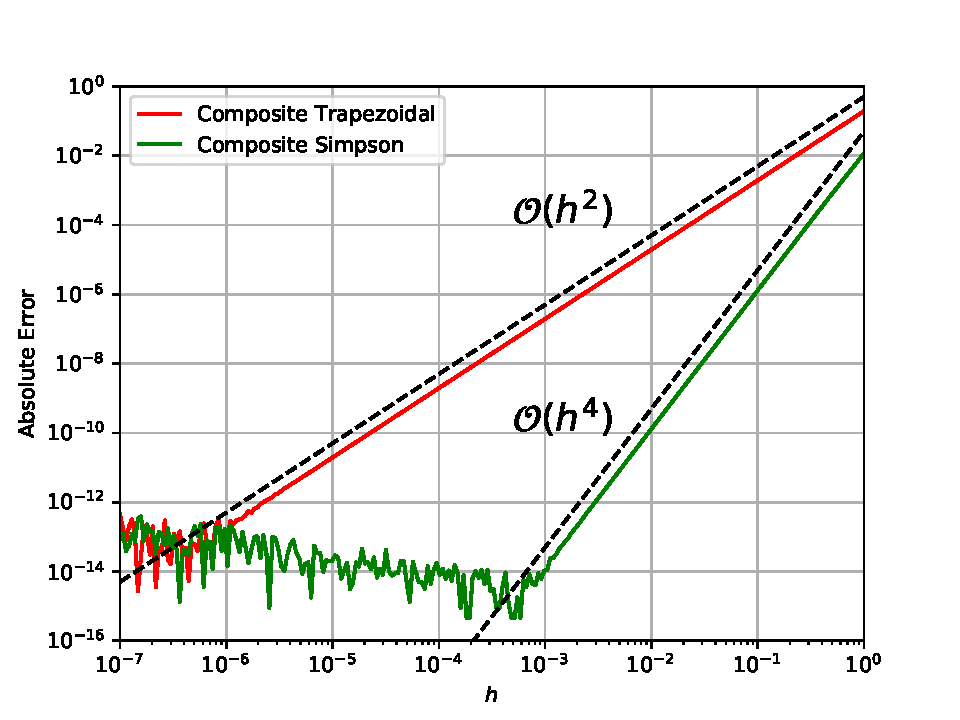
\includegraphics[width=0.65\textwidth]{compositenewtoncotes}
\caption{Comparison of the composite trapezoidal and Simpson's rules for $\int_{-1}^1e^x\ud x$. The dashed black lines are representative second- and fourth-order scalings.}
\label{figure:CompositeNewtonCotes}
\end{center}
\end{figure}

%\subsection{Adaptive Quadrature}
%\subsection{Euler--Maclaurin Summation Formula}

\section{Richardson Extrapolation}

Richardson extrapolation~\cite{Richardson-210-459-11} is an algorithm designed to transform, in certain cases, the asymptotic expansion of the error in a formula into a systematic method that exploits structure of the asymptotic expansion in order to provide a more accurate result. The result is known as an {\em extrapolant} as it is usually beyond reach. Suppose we are interested in the quantity $A$ and we can approximate it by $A_h$, where $h>0$ is some tuneable parameter. Furthermore, suppose we are aware of the asymptotic expansion:
\[
A_h = A + c_1h + c_2h^2 + \cdots + c_nh^n + \OO(h^{n+1}),\quad{\rm as}\quad h\to0.
\]
Such an expansion is motivated by Taylor's theorem, and as such Richardson extrapolation can improve the approximation of derivatives by finite differences and the approximation of integrals by Newton--Cotes quadrature. The next step is to assume we are in the r\'egime where $h$ is truly small, such that we only incur a small error in setting:
\begin{equation}\label{eq:RichardsonExtrapolation}
\hat{A} + \hat{c}_1h + \hat{c}_2h^2 + \cdots + \hat{c}_nh^n = A_h.
\end{equation}
To solve for the $n$ unknowns $\hat{A}$ and $\hat{c}_k$ for $k=1,\ldots,n$, we use $n+1$ distinct values of $h$ to setup and solve the linear system:
\begin{equation}\label{eq:Vandermonde}
\begin{bmatrix}
1 & h_0 & \cdots & h_0^n\\
1 & h_1 & \cdots & h_1^n\\
\vdots & \vdots & \ddots & \vdots\\
1 & h_n & \cdots & h_n^n\\
\end{bmatrix}
\begin{bmatrix} \hat{A}\\\hat{c}_1\\\vdots\\\hat{c}_n\end{bmatrix}
=
\begin{bmatrix} A_{h_0}\\A_{h_1}\\\vdots\\A_{h_n}\end{bmatrix}.
\end{equation}
The matrix in~\eqref{eq:Vandermonde} is known as the Vandermonde matrix. While a direct method would require $\OO(n^3)$ flops for the solution of the unknowns $\hat{A}$ and $\hat{c}_k$, recall that we are only interested in the extrapolant $\hat{A}$: the unknowns $\hat{c}_k$ are auxiliary variables introduced to satisfy the asymptotic expansion. Thus, we may intuitively expect to only require $\OO(n^2)$ operations to only solve for the unknown $\hat{A}$.

We turn to an already familiar tool for the solution. First, we rewrite~\eqref{eq:RichardsonExtrapolation} as follows:
\[
\hat{c}_1 + \hat{c}_2h + \cdots + \hat{c}_nh^{n-1} = \dfrac{A_h-\hat{A}}{h}.
\]
Since the left-hand side is a degree-$(n-1)$ polynomial in $h$, the $n^{\rm th}$ Newton divided difference will annihilate it:
\[
0 \equiv \delta^{(n)}[h_0,\ldots,h_n]\pr(\hat{c}_1 + \hat{c}_2h + \cdots + \hat{c}_nh^{n-1}) = \delta^{(n)}[h_0,\ldots,h_n]\pr(\dfrac{A_h-\hat{A}}{h}).
\]
Since the unknown $\hat{A}$ is a constant (in terms of the parameter $h$), we may isolate for it as follows:
\[
\hat{A} = \dfrac{\displaystyle\delta^{(n)}[h_0,\ldots,h_n]\pr(\frac{A_h}{h})}{\displaystyle\delta^{(n)}[h_0,\ldots,h_n]\pr(\frac{1}{h})}.
\]
Since Newton divided differences can be computed in $\OO(n^2)$ by organizing the calculation in a tableau, we now have a fast method for computing Richardson extrapolants.

\begin{example}
Let us approximate $\pi$ by inscribed polygons in the unit circle. For a regular $n$-gon, the circumference is $2n\sin(\pi/n) \le 2\pi$, so let $C_n = n\sin(\pi/n) \le \pi$ be half the circumference. Indeed, $C_2 = 2\sin(\pi/2) = 2$. Furthermore, we can compute a sequence of circumferences recursively:
\begin{align*}
C_{2n} = 2n\sin(\pi/2n) & = 2n\sqrt{\frac{1}{2}(1-\cos(\pi/n))},\\
& = 2n\sqrt{\frac{1}{2}\left(1-\sqrt{1-\sin^2(\pi/n)}\right)},\\
& = 2n\sqrt{\frac{1}{2}\left(1-\sqrt{1-(C_n/n)^2}\right)}.
\end{align*}
Since this expression is sensitive to rounding errors, we rewrite it as:
\[
C_{2n} = \dfrac{C_n\sqrt{2}}{\sqrt{1+\sqrt{1-(C_n/n)^2}}}.
\]
If we let $h = 1/n^2$, then:
\[
C_{1/\sqrt{h}} = A_h = \dfrac{\sin(\pi \sqrt{h})}{\sqrt{h}} = \pi - \dfrac{\pi^3h}{6} + \dfrac{\pi^5h^2}{120}+\cdots+.
\]

Table~\ref{table:Richardson1} shows the result of applying Richardson extrapolation when $h = 1/n^2$ for $n=2,4,8,\ldots.$ Bold digits represent correct values when approximating $\pi$.
\begin{table}[htp]
\caption{Richardson extrapolation of the circumference of an $n$-gon.}
\begin{center}
\begin{tabular}{rll}
\hline
$n$ & $C_n$ & Richardson Extrapolants\\
\hline
$2$ & $2.000000000000000$ & $2.000000000000000$\\
$4$ & $2.8284271247461903$ & ${\bf 3.1}04569499661587$\\
$8$ & ${\bf 3}.0614674589207187$ & ${\bf 3.141}4527750222714$\\
$16$ & ${\bf 3.1}21445152258053$ & ${\bf 3.141592}5775443454$\\
$32$ & ${\bf 3.1}365484905459398$ & ${\bf 3.14159265358}3072$\\
$64$ & ${\bf 3.14}0331156954754$ & ${\bf 3.14159265358979}44$\\
$128$ & ${\bf 3.141}277250932774$ & ${\bf 3.14159265358979}5$\\
$256$ & ${\bf 3.1415}138011443027$ & ${\bf 3.14159265358979}5$\\
\hline
$+\infty$ & ${\bf 3.141592653589793\cdots}$ & ${\bf 3.141592653589793\cdots} =\pi$\\
\hline
\end{tabular}
\end{center}
\label{table:Richardson1}
\end{table}%
\end{example}

\section{Gaussian Quadrature}

While the family of (composite) Newton--Cotes quadrature formul\ae~take equispaced nodes, if we relax this restriction, then the resulting quadrature formula can be more accurate. Consider the problem of choosing the nodes and weights in the quadrature formula:
\[
\int_a^bf(x)w(x)\ud x \approx \sum_{k=1}^n w_kf(x_k)
\]
so that the rule is exact for polynomials of degree as high as possible. Being optimistic, with $n$ nodes and weights at our disposal, we hope it will satisfy $2n$ exactness conditions of the type:
\[
\int_a^b x^m w(x)\ud x = \sum_{k=1}^n w_k x_k^m,\quad{\rm for}\quad m=0,\ldots,2n-1.
\]
The word ``hope'' was used in the previous sentence because these last equations, while linear in the weights, are nonlinear in the nodes. Hence, these might {\em a priori} be complex numbers or even real numbers outside of $(a,b)$. In either case, the quadrature formula would be useless. Fortunately, the following theorem relates the nodes of the Gaussian quadrature formula to the zeros of the orthogonal polynomials, and by construction, it follows that these nodes are located within the interval $(a,b)$.

\begin{theorem}\label{theorem:Gaussnodesandweights}
Let $w\ge0$ be a non-negative weight function on $[a,b]$ and let $a,b\in\R$. Then:
\begin{enumerate}
\item the nodes of the Gaussian quadrature formula are the zeros of the orthogonal polynomial $\pi_n$ with respect to $L^2([a,b],w(x)\ud x)$;
\item The formula:
\[
\int_a^bf(x)w(x)\ud x = \sum_{k=1}^n w_kf(x_k),
\]
is exact for every $f\in\P_{2n-1}$; and,
\item The weights $w_k>0$ for $k=1,\ldots,n$.
\end{enumerate}
\end{theorem}
\begin{proof}
Let $\pi_n$ be the degree-$n$ orthogonal polynomial with respect to $L^2([a,b],w(x)\ud x)$, and let $x_1,\ldots,x_n$ be its zeros. If $f\in\P_{2n-1}$, there exists $q,r\in\P_{n-1}$ such that $f = q\pi_n + r$. Since $x_k$ are the roots of $\pi_n$, it follows that $f(x_k) = r(x_k)$ for $k=1,\ldots,n$. Hence:
\[
r(x) = \sum_{k=1}^n \ell_{n,k}(x) f(x_k),
\]
where $\ell_{n,k}(x)\in\P_{n-1}$ for $k=1,\ldots,n$ are the Lagrange basis polynomials through the roots of $\pi_n$. We integrate to obtain:
\begin{align*}
\int_a^b f(x)w(x)\ud x & = \int_a^b\left(q(x)\pi_n(x)+r(x)\right)w(x)\ud x,\\
& = \int_a^b q(x)\pi_n(x)w(x)\ud x + \int_a^br(x) w(x)\ud x,\\
& = 0 + \sum_{k=1}^nw_kf(x_k),
\end{align*}
where the $q\pi_n$ integrates to $0$ by orthogonality and where:
\[
w_k = \int_a^b \ell_{n,k}(x)w(x)\ud x,\quad{\rm for}\quad k=1,\ldots,n.
\]
Clearly, 1.~holds by applying Theorem~\ref{theorem:OPzeros}, 2.~holds without loss of generality, and 3.~holds by repeating the argument with the alternative interpolant:
\[
f(x) = q(x)\pi_n(x) + \sum_{k=1}^n\left[\ell_{n,k}(x)-\ell_{n,k}^2(x)\right]f(x_k) + \sum_{k=1}^n\ell_{n,k}^2(x)f(x_k),\in\P_{2n-1},
\]
and since $\ell_{n,k}-\ell_{n,k}^2$ is zero at each of the roots, $\pi_n$ is a divisor.
\end{proof}

\begin{remark}
Note that due to the limiting form of the Lagrange basis polynomials:
\begin{equation}\label{eq:GQweights}
w_k = \int_a^b \dfrac{\tilde{\pi}_n(x)w(x)\ud x}{\tilde{\pi}_n'(x_k)(x-x_k)},\quad{\rm for}\quad k=1,\ldots,n.
\end{equation}
To find a more convenient expression for the weights $w_k$, recall the Christoffel--Darboux formula~\eqref{eq:ChristoffelDarboux}:
\[
\sum_{j=0}^{n-1}\tilde{\pi}_j(x)\tilde{\pi}_j(y) = \sqrt{\beta_n}\dfrac{\tilde{\pi}_n(x)\tilde{\pi}_{n-1}(y) - \tilde{\pi}_{n-1}(x)\tilde{\pi}_n(y)}{x-y}.
\]
If we let $y=x_k$ in~\eqref{eq:ChristoffelDarboux}, where $x_k$ is a zero of $\pi_n$, then:
\begin{equation}\label{eq:ChristoffelDarbouxRoot}
\sum_{j=0}^{n-1}\tilde{\pi}_j(x)\tilde{\pi}_j(x_k) = \sqrt{\beta_n}\dfrac{\tilde{\pi}_n(x)\tilde{\pi}_{n-1}(x_k)}{x-x_k}.
\end{equation}
Multiplying by $w(x)$, integrating over $[a,b]$, and comparing the result with~\eqref{eq:GQweights}, we find:
\begin{align*}
1 & = \int_a^b \tilde{\pi}_0(x)\tilde{\pi}_0(x)w(x)\ud x = \int_a^b \tilde{\pi}_0(x)\tilde{\pi}_0(x_k)w(x)\ud x = \int_a^b \sum_{j=0}^{n-1}\tilde{\pi}_j(x)\tilde{\pi}_j(x_k)w(x)\ud x\\
& = \sqrt{\beta_n}\tilde{\pi}_{n-1}(x_k)\int_a^b\dfrac{\tilde{\pi}_n(x)w(x)\ud x}{x-x_k} = \sqrt{\beta_n}\tilde{\pi}_{n-1}(x_k)\tilde{\pi}_n'(x_k)w_k.
\end{align*}
On the other hand, if we take the limit as $x\to x_k$ in~\eqref{eq:ChristoffelDarbouxRoot}, then:
\begin{equation}\label{eq:ChristoffelDarbouxLimit}
\sum_{j=0}^{n-1}[\tilde{\pi}_j(x_k)]^2 = \sqrt{\beta_n}\tilde{\pi}_n'(x_k)\tilde{\pi}_{n-1}(x_k).
\end{equation}
Comparing these two equations, we find:
\begin{equation}\label{eq:GQweights2}
w_k^{-1} = \sum_{j=0}^{n-1}[\tilde{\pi}_j(x_k)]^2,\quad{\rm for}\quad k=1,\ldots,n.
\end{equation}
\end{remark}

This theorem gives the nodes of the Gaussian quadrature formula as the roots of the associated orthogonal polynomials. The following theorem, motivated by Theorems~\ref{theorem:threetermrecurrence},~\ref{theorem:ChristoffelDarboux}, and~\ref{theorem:Gaussnodesandweights}, represents the nodes of Gaussian quadrature (zeros of orthogonal polynomials) as the eigenvalues of a special matrix, and the weights are given in terms of the first components of the eigenvectors.
\begin{theorem}\label{theorem:JacobiMatrix}
Let $\alpha_n$ and $\beta_n$ be the recurrence coefficients defined in Theorem~\ref{theorem:threetermrecurrence} for the monic orthogonal polynomials $\hat{\pi}$:
\[
\alpha_n = \dfrac{\langle \hat{\pi}_n,x\hat{\pi}_n\rangle}{\langle\hat{\pi}_n,\hat{\pi}_n\rangle}\quad{\rm and}\quad \beta_n = \dfrac{\langle \hat{\pi}_n,\hat{\pi}_n\rangle}{\langle\hat{\pi}_{n-1},\hat{\pi}_{n-1}\rangle}.
\]
The eigenvalues of the symmetric {\bf Jacobi matrix}:
\[
J := \begin{bmatrix}
\alpha_0 & \sqrt{\beta_1}\\
\sqrt{\beta_1} & \alpha_1 & \sqrt{\beta_2}\\
& \ddots & \ddots & \ddots\\
& & \sqrt{\beta_{n-2}} & \alpha_{n-2} & \sqrt{\beta_{n-1}}\\
& & & \sqrt{\beta_{n-1}} & \alpha_{n-1}\\
\end{bmatrix},
\]
are the nodes of the Gaussian quadrature formula. Furthermore, let $\mu_0 = \int_a^b w(x)\ud x$ and let $q_k$ denote the $k^{\rm th}$ normalized eigenvector of the Jacobi matrix $J$. Then the weights are given by:
\begin{equation}\label{eq:GQweights3}
w_k = [q_k]_1^2\mu_0.
\end{equation}
\end{theorem}
\begin{proof}
We write the recurrence relation:
\[
\hat{\pi}_{n+1}(x) = (x-\alpha_n)\hat{\pi}_n(x) - \beta_n\hat{\pi}_{n-1}(x),
\]
in matrix form for $k=0,\ldots,n-1$, and obtain:
\[
\hat{J}\begin{bmatrix} \hat{\pi}_0\\\hat{\pi}_1\\\vdots\\\hat{\pi}_{n-1}\end{bmatrix}
=
x\begin{bmatrix} \hat{\pi}_0\\\hat{\pi}_1\\\vdots\\\hat{\pi}_{n-1}\end{bmatrix}
-
\begin{bmatrix} 0\\0\\\vdots\\\hat{\pi}_n\end{bmatrix},
\]
where:
\[
\hat{J} = \begin{bmatrix}
\alpha_0 & 1\\
\beta_1 & \alpha_1 & 1\\
& \ddots & \ddots & \ddots\\
& & \beta_{n-2} & \alpha_{n-2} & 1\\
& & & \beta_{n-1} & \alpha_{n-1}\\
\end{bmatrix}.
\]
Thus, $\tilde{\pi}_n(x_k)$ is zero if and only if $x_k$ is an eigenvalue of the Jacobi matrix $J\tilde{\pi}(x_k) = x_k\tilde{\pi}(x_k)$. The matrix $J$ and $\hat{J}$ only differ in the diagonal similarity transformation $J = S\hat{J}S^{-1}$, where:
\[
S = \begin{bmatrix}
1\\
& 1/\sqrt{\beta_1}\\
& & \ddots\\
& & & 1/\sqrt{\beta_1\cdots\beta_{n-1}}
\end{bmatrix}.
\]
Since the eigenvectors $q_k$ are normalized, $\langle q_k, q_k\rangle = 1$, they can be written as:
\[
q_k = \left(\sum_{j=0}^{n-1}[\tilde{\pi}_j(x_k)]^2\right)^{-1/2}\begin{bmatrix}\tilde{\pi}_0(x_k)\\\tilde{\pi}_1(x_k)\\\vdots\\\tilde{\pi}_{n-1}(x_k)\end{bmatrix}
\]
Since $\tilde{\pi}_0(x_k) \equiv \mu_0^{-1/2}$, the weights~\eqref{eq:GQweights2} are given by~\eqref{eq:GQweights3}.
\end{proof}

\begin{remark}
While $J$ and $\hat{J}$ are similar matrices and therefore have the same spectrum, it is computationally better to work with the symmetric Jacobi matrix $J$.
\end{remark}

\begin{example}
The monic Legendre polynomials satisfy the recurrence relation:
\[
\hat{P}_{n+1}(x) = x\hat{P}_n(x) - \dfrac{n^2}{4n^2-1}\hat{P}_{n-1}(x).
\]
Therefore, the zeros of the Legendre polynomials are the eigenvalues of the matrix:
\[
J_{\rm Legendre} =  \begin{bmatrix}
0 & \sqrt{\tfrac{1}{3}}\\
\sqrt{\tfrac{1}{3}} & 0 & \sqrt{\tfrac{4}{15}}\\
& \ddots & \ddots & \ddots\\
& & \sqrt{\tfrac{(n-2)^2}{4(n-2)^2-1}} & 0 & \sqrt{\tfrac{(n-1)^2}{4(n-1)^2-1}}\\
& & & \sqrt{\tfrac{(n-1)^2}{4(n-1)^2-1}} & 0\\
\end{bmatrix},
\]
Since $\mu_0 = \int_\I\ud x = 2$, for $n=10$, for example, we can reproduce the Table~\ref{table:GaussLegendre}.
\begin{table}[htp]
\caption{Ten nodes and weights of Gauss quadrature with respect to $L^2(\I,\ud x)$.}
\begin{center}
\begin{tabular}{rll}
\hline
$k$ & Nodes & Weights\\
\hline
$1$ & $-0.9739065285171719$ & $0.06667134430868686$\\
$2$ & $-0.8650633666889844$ & $0.14945134915058303$\\
$3$ & $-0.6794095682990244$ & $0.21908636251598385$\\
$4$ & $-0.4333953941292472$ & $0.2692667193099954$\\
$5$ & $-0.14887433898163138$ & $0.29552422471475015$\\
$6$ & $0.1488743389816315$ & $0.2955242247147527$\\
$7$ & $0.4333953941292473$ & $0.26926671930999535$\\
$8$ & $0.6794095682990242$ & $0.21908636251598348$\\
$9$ & $0.8650633666889844$ & $0.14945134915058114$\\
$10$ & $0.9739065285171715$ &  $0.06667134430868785$\\
\hline
\end{tabular}
\end{center}
\label{table:GaussLegendre}
\end{table}%
Notice the symmetry in the nodes and weights.
\end{example}

Now that we can compute general Gaussian quadrature rules, it is interesting to see how quickly they converge. For this, we have the following theorem.

\begin{theorem}\label{theorem:GaussError}
Let $f\in C^{2n}([a,b])$. Then $\exists \xi\in(a,b)$ such that:
\[
\int_a^bf(x)w(x)\ud x - \sum_{k=1}^nw_kf(x_k) = \langle\hat{\pi}_n,\hat{\pi}_n\rangle\dfrac{f^{(2n)}(\xi)}{(2n)!}.
\]
\end{theorem}

\section{Monte Carlo Integration}

This method approximates the value of an integral by the average of the integrand evaluated at many random points. It is only practical for high-dimensional integrals.

Given $f\in C([a,b])$, we wish to approximate:
\[
I = \int_a^b f(x)\ud x.
\]
Suppose $x_i$ are independent samples from the uniform distribution on $[a,b]$. Then, with $N$ such random points, an approximation to $I$ is:
\[
I_N = \dfrac{b-a}{N}\sum_{i=1}^Nf(x_i).
\]
We now compute two statistics, the expectation $E(I_N)$ and the standard deviation $\sigma(I_N)$:
\begin{align*}
E(I_N) & = \dfrac{b-a}{N}\sum_{i=1}^N E(f),\\
& = (b-a)E(f),\\
& = (b-a)\dfrac{\int_a^bf(x)\ud x}{b-a},\\
& = I.
\end{align*}
This is promising. Next, we compute the variance of $I_N$:
\begin{align*}
\var\left(\dfrac{b-a}{N}\sum_{i=1}^N f(x_i)\right) & = \dfrac{(b-a)^2}{N^2}\var\left(\sum_{i=1}^Nf(x_i)\right)\\
& = \dfrac{(b-a)^2}{N^2}N\var(f).
\end{align*}
Recall that $\var(f) = E(f^2)-E(f)^2$. Then:
\[
\sigma(I_N) = (\var(I_N))^{1/2} = \dfrac{(b-a)(E(f^2)-I^2)^{1/2}}{\sqrt{N}}.
\]
Thus, the standard deviation, which measures the deviation from the expected value and thus is in some sense the ``error'' of the approximation, behaves like $N^{-1/2}$. Since the error of the trapezoidal rule is $\OO(N^{-2})$ for $f\in C^2$, the Monte Carlo method is not competitive for one-dimensional integrals. However, in $d$ dimensions, the error of the trapezoidal rule is $\OO(N^{-2/d})$ while that of the Monte Carlo method is still $\OO(N^{-1/2})$, independent of $d$! Hence, when $d>4$, the Monte Carlo method is more efficient than the trapezoidal rule. As an added bonus, the Monte Carlo method is insensitive to endpoint singularities or cusps of the integrand.

\begin{comment}

In the above description of the Monte Carlo method, we employed the uniform distribution. This may not be the best. Suppose we choose the distribution $p(x)>0$, which of course satisfies:
\[
\int_a^b p(x)\ud x = 1.
\]
Then:
\[
\int_a^bf(x)\ud x = \int_a^bg(x)p(x)\ud x,\qquad g(x) = \dfrac{f(x)}{p(x)}.
\]
We can now define the approximation:
\[
I_N = \dfrac{1}{N}\sum_{i=1}^Ng(x_i),
\]
where $x_i$ has probability distribution $p$. It follows that:
\begin{align*}
E(I_N) & = \dfrac{1}{N}\sum_{i=1}^N E(g) = E(g),\\
& = \int_a^bg(x)p(x)\ud x = \int_a^bf(x)\ud x = I.
\end{align*}
Now:
\begin{align*}
\var(I_N) & = \dfrac{1}{N}\var(g) = \dfrac{1}{N}\left(E(g^2)-E(g)^2\right),\\
& = \dfrac{1}{N}\left[\int_a^bg(x)^2p(x)\ud x - I^2\right] = \dfrac{1}{N}\left[\int_a^b\dfrac{f(x)^2}{p(x)}\ud x - I^2\right].
\end{align*}
Finally:
\[
\sigma(I_N) = \dfrac{1}{\sqrt{N}}\left[\int_a^b\dfrac{f(x)^2}{p(x)}\ud x - I^2\right]^{1/2}.
\]
While the standard deviation is still $\OO(N^{-1/2})$ in general, the constant multiplying $N^{-1/2}$ can be smaller if $p$ is chosen properly.

%\subsection{Antithetic Variates}
%Using antithetic sampling is a method of variance reduction for Monte Carlo methods. For every sample taken $x_i$ , its {\em antithesis} $y_i$ is also used. 

\end{comment}

\section{Problems}

\begin{enumerate}

\item Finite differences have many applications. Consider the first-order ordinary differential equation:
\[
y' = f(t,y),\quad y(0) = y_0.
\]
This is an initial-value problem (IVP).
\begin{enumerate}
\item Use the forward and backward difference formul\ae~to derive Euler's forward and backward approximations:
\[
y(t+h) \approx y(t) + hf(t,y(t)), \quad{\rm and}\quad y(t+h) \approx y(t) + hf(t+h,y(t+h)).
\]
\item Use the forward/backward Euler methods to write a time-stepping code that solves the IVP $y' = y$ with $y(0) = 1$ for $t\in[0,1]$. Keep track of your results in the form of a table, recording the step size $h$ and the final values $y_{\rm Approx}(1) \approx e$.
\item Refine your time-stepping estimates using Richardson extrapolation on the table values. What is your best approximation to $e$?
\end{enumerate}

\item Use the rules of evaluation at dual numbers to determine $f'(1)$ for $f(x) = \sqrt{\sin(e^x)+\cos(x^2)}$, i.e. evaluate $f(1+\varepsilon) = f(1) + f'(1)\varepsilon$.

\item Prove Theorem~\ref{theorem:TrapezoidalIMVTError}.

\item Go to {\tt https://www.wolframalpha.com}, and ask ``What is the rubber ducky curve?'' Use a composite Newton--Cotes quadrature formula to estimate the area enclosed by the parametric curve:
\[
{\rm Area} = \dfrac{1}{2}\int_0^{2\pi}r^2(\theta)\ud\theta,
\]
where $r(\theta) = \sqrt{x^2(\theta)+y^2(\theta)}$. Tabulate the number of points you use and the resulting approximation. {\em And no, the answer is not ``one duck.'' If you don't want to do the duck, go to {\tt https://gist.github.com/simcop2387/5493206} for a full list of Wolfram's curves. Be sure to choose one that is periodic and doesn't involve the Heaviside step function, i.e. they must be plotted on $[0,2\pi)$, otherwise low accuracy will result. Moose, pig, lion, elephant, mammoth, bunny, first cat, Ferrari, Statue of Liberty, etc\ldots, all work. If you are not interested in typing in the formula, check UM Learn for the {\sc Julia} script {\tt duck.jl} for $x(\theta)$ and $y(\theta)$.}

%\item An infinite number of pure mathematicians walk into a bar. The first one asks the bartender for a pint; the second asks for half a pint, and the third asks for another quarter. Bitter and jaded from his/her pure mathematics career path, the bartender pours two pints for all of them to share. A few minutes later, an infinite number of applied mathematicians walk into the same bar. Again, the thirstiest asks the bartender for a pint, but the second asks for only a {\em quarter} pint, and the third asks for a {\em ninth}. In the name of expediency, the bartender pulls out a pen and a sheet of paper and uses Richardson extrapolation to estimate how much beer to pour for the applied mathematicians. What does s/he write down?

\item Hermite polynomials are orthogonal polynomials with respect to $L^2(\R,e^{-x^2}\ud x)$. They satisfy the following recurrence:
\[
H_{n+1}(x) = 2x H_n(x) - 2nH_{n-1}(x), \quad H_0(x) = 1,\quad H_1(x) = 2x.
\]
\begin{enumerate}
\item Derive the recurrence for the {\em monic} Hermite polynomials $\hat{H}_n(x)$.
\item Calculate $\mu_0 = \int_\R e^{-x^2}\ud x$ by writing $\mu_0^2 = \int_\R e^{-x^2}\ud x\times \int_\R e^{-y^2}\ud y$ and using a variable transformation to polar coordinates ($x=r\cos\theta$, $y=r\sin\theta$, and $\ud x\ud y = r\ud r\ud\theta$).
\item Use the above to construct the Jacobi matrix $J_{\rm Hermite}$ and use Theorem~\ref{theorem:JacobiMatrix} to calculate the nodes and weights of Gauss--Hermite quadrature of order $10$.
\end{enumerate}

%\item Prove Theorem~\ref{theorem:GaussError}. {\em Hint: integrate the Hermite interpolating formula}.

\item The function $\displaystyle B_d(s) = \int_{[0,1]^d} (x_1^2+\cdots+x_d^2)^{s/2}\ud x_1\cdots\ud x_d = \int_{[0,1]^d} \norm{x}_2^s\ud^dx$ is called a box integral. Box integrals appear in Jellium physics. Write a Monte Carlo integrator to approximate box integrals. Compare your results with:
\begin{enumerate}
\item $B_4(-2) = \pi\log\pr(2+\sqrt{3}) -2G -\dfrac{\pi^2}{8}$, where $G = 0.91596\,55941\,77219\ldots$ is Catalan's constant; and,
\item $B_d(1) \sim \sqrt{\dfrac{d}{3}}\left(1-\dfrac{1}{10d}\right)$ for $d=10,1\,000,$ and $1\,000\,000$.
\end{enumerate}

\end{enumerate}